% !TEX encoding = UTF-8 Unicode
%
% An essay from Jonas Tobias Hopusch,
% partially using a latex template by Professor Hans-Georg Eßer
%
% SPDX-FileCopyrightText: 2023 Jonas Tobias Hopusch <git@jotoho.de>
% SPDX-License-Identifier: CC-BY-SA-4.0
%

\documentclass[a4paper,numbers=withenddot,11pt]{scrartcl}
\usepackage{fontspec}\usepackage[ngerman]{babel}
\usepackage{blindtext}\usepackage{url}
\usepackage{listings}\lstset{basicstyle=\footnotesize\ttfamily,breaklines=true}
\usepackage{setspace}\setstretch{1.1}
\usepackage[hidelinks]{hyperref}
\usepackage{graphicx}

\newcommand\modulname{Skriptsprachen}
\newcommand\autorname{Jonas Tobias Hopusch}
\title{Entwicklung einer CLI Anwendung -- einfaches Linux Moddingwerkzeug mithilfe fuse-overlayfs}
\author{\autorname\\ FH Südwestfalen \\[5mm] Schriftliche Ausarbeitung im Modul\\ „\modulname“}
\parindent0pt\parskip6pt
\clubpenalty = 10000
\widowpenalty = 10000
\displaywidowpenalty = 10000

\begin{document}

\maketitle
\tableofcontents

Das Projektrepositorium auf GitHub finden Sie hier:\\
\href{https://github.com/jotoho/tes-moddingoverlay}{github.com/jotoho/tes-moddingoverlay}

Sollte das Repositorium auf privat gestellt sein und sie es einsehen wollen,
können Sie mich per E-Mail an \href{mailto:git@jotoho.de}{git@jotoho.de} kontaktieren.\\
Um Ihnen ggf. Einsicht geben zu können, benötige ich Ihren GitHub-Nutzernamen.

\section{Motivation}

Als ich erfuhr, dass wir für unser Projekt im Kurs Skriptsprachen die Option haben,
ein Admin- oder CLI-Werkzeug zu schreiben, habe ich mir einige Tage gedanken gemacht,
was ich mir sinnvoll vornehmen konnte.

Während ich einfach irgendein Standardbeispiel für Werkzeuge oder Spiele hätte nehmen
können, habe ich in der Vergangenheit die Erfahrung gemacht, dass solche Projekte
einmal programmiert werden und danach metaphorisch in der Schublade verschwinden und
dann nie wieder benutzt oder angeschaut werden.

Da klar war, dass in dieses Projekt einige Tage Arbeit hineinfließen würden,
wollte ich idealerweise etwas schreiben, das auch nach diesem Semester weiterhin
nützlich sein könnte.

Als langjähriger Nutzer des Linux-Betriebssystems habe ich die Erfahrung gemacht,
dass es für viele, auch anspruchsvolle, Aufgaben bereits erfolgreiche und
zuverlässige Werkzeuge gibt.

In einem Feld habe ich allerdings schon häufiger das Problem der Programmkompatiblität
unter Linux gehabt: Videospiele.\\
Um genau zu sein, die Mittel eines Spielers, ein Spiel, welches er besitzt,
mithilfe von spielergemachten Mods (kurz für engl. Modification) einfach zu installieren
und verwalten.

Während WINE und Proton es zwar inzwischen möglich gemacht haben, die meisten
Windowsspiele auch unter Linux spielen zu können, habe ich über die Jahre häufig
versucht Modwerkzeuge wie Vortex (von Nexus Mods) und Mod Organizer 2 unter Linux
ans laufen zu bringen und immer sehr große Probleme gehabt.

Zusätzlich zu den vielen Komfortfunktionen, die diese Werkzeuge unter Windows bringen,
wie erleichtertes Herunterladen und Aktualisieren, gibt es einen wichtigen Aspekt
für jedes Moddingvorhaben mit mehr als einer handvoll Mods:\\
Sowohl Vortex als auch Mod Organizer 2 installieren Mods nicht direkt in das
Spieleverzeichnis, sondern je in einen eigenen Ordner, um sie voneinander zu isolieren.
Von dort werden sie dann via soft links, hard links oder kopieren (Vortex) oder
ein virtuelles Dateisystem (VFS in Mod Organizer 2) zum Spielestart in die Spieldaten
injiziert.

Dies ist unglaublich wichtig, da es verhindert, dass bei Konflikten zwischen Mods die
Installationreihenfolge der Mods entscheidet, welche Mod gewinnt und es ermöglicht
Mods nachträglich zu deinstallieren oder mit einer anderen (neueren) Version auszutauschen.

Als konsequenz von großen technischen Problemen habe ich viel Zeit verloren und schon
mehrmals eine Spielinstallation und die dazugehörigen Spielstände aufgeben müssen, weil
die Werkzeuge unter WINE und Proton versagt haben.

In meiner verzweifelten Suche nach einer Möglichkeit die Spiele zuverlässig auf Linux
ans laufen zu bekommen und zu modden, bin ich vor langer Zeit auf reddit auf das overlay
file system auf Linux aufmerksam geworden.\\
(Da dies inzwischen Jahre her ist, weiß ich leider nicht mehr,
welcher Redditbeitrag es war und ob er overlayfs im Kontext von Modding erwähnte
oder ob die Idee es so einzusetzen von mir stammt.)

Dazu kommen meine Erfahrungen mit der open source engine reimplementierung OpenMW
für `The Elder Scrolls III: Morrowind'.
OpenMW ist ein Community-Projekt welches es Spielern erlaubt Morrowinddateien
zu laden und das Spiel in einer moderneren und stabileren Engine zu spielen.
Ich nutze OpenMW schon seit Jahren für das Spielen von Morrowind, da es zusätzlich
zu all den algemeinen Vorteilen, von denen auch Windowsspieler profitieren,
auch nativ unter Linux läuft.
Ein weniger bekanntes Feature von OpenMW, welches vor kurzem einfacher zu verwenden
wurde, ist die Möglichkeit mehrere Quellverzeichnisse zu spezifizieren aus denen
Spieledateien und Plugins geladen werden.
Dies erlaubte mir, für das Basisspiel und für jede Mod jeweils einen dedizierten
Ordner zu erstellen und die so einzeln verwalten und aktualisieren zu können.
Während das immernoch etwas mehr Aufwand war, als mit einem vollständigen
Mod Manager, ist das immernoch mehr als gut genug um sicher und zuverlässig
mit mehreren duzend Mods zu spielen. (Aktuell \~{}75 mods)

Ich nahm mir also vor, als Projekt für diese Ausarbeitung, ein rudimentäres
Moddingwerkzeug für meine Verwendung auf Linux zu entwickeln, welches
die Taktik des VFS-Einspeisens von Moddateien von Mod Organizer
mit der user-space implementierung von overlayfs (fuse-overlayfs)
kombiniert um eine ähnliche Erfahrung beim modden anderer Spiele zu haben,
wie mit OpenMW data directories.

\section{Projektbeschreibung}

Das von mir für diese Ausarbeitung programmierte Modding-Werkzeug,
bekam von mir den provisorischen Namen `modfs' und wird im folgenden so genannt.

modfs als Werkzeug hat die Aufgabe, mods auf Nutzeranfrage aus der
Ordnerstruktur der Instanz herauszulesen und automatisch im overlayfs zu
konfigurieren, welches dann über das Spielverzeichnis gelegt wird.

Das gestartete Spiel und alle anderen Anwendungen bekommen bei aktivem
Dateisystem das Verzeichnis so angezeigt, als wären alle Mods in Reihenfolge
der Priorität über das unmodifizierte Spiel herüberkopiert worden.

Der Vorteil für den Benutzer liegt darin, dass die Mods in Wahrheit
allerdings weiterhin voneinander isoliert sind, keine Dateien verloren gehen
und Änderungen an Dateien im Spieleverzeichnis sich nicht auf die Originale durchschlagen,
sondern der neue Stand solcher Dateien in einem eigenen Overflow-Ordner
gespeichert werden.
Von dort kann der Nutzer später entscheiden, ob er die Änderungen zu einer
eigenständigen Mod (im Sinne von modfs) machen oder löschen will.

Anders als bei Mod Organizer 2 wird das VFS nicht nur für ein einziges
Programm und nur für dessen Laufzeit angewendet, sondern läuft für alle
Anwendungen gleich, bis es beendet wird.
(Durch den `modfs.py deactivate'-Befehl, einen Systemneustart oder anderswie)

Um zu erlauben, dass mehrere Spiele auf einmal gemoddet sein können,
geht modfs von einem Instanzen-modell aus.
Das heißt, man kann modfs in einem leeren Verzeichnis mit dem Befehl
`modfs init' aufrufen und das Programm generiert das allernötigste an
Dateien und Verzeichnissen um funktionieren zu können.
Die Informationen zu einer gewissen Modsammlung wird so getrennt vom
Programm gehalten und eine Installation von modfs kann beliebig viele
Spiele auf einmal bedienen.

modfs geht stets davon aus, dass es aus dem root-Verzeichnis der Instanz
aufgerufen wird oder den Ort der tatsächlichen Instanz per `--instance'
CLI-Parameter mitgeteilt bekommt.

\subsection{Befehlsübersicht}

Dies ist nur ein Ausschnitt der wichtigsten Befehle / Befehlskombinationen.
Nutzer können jederzeit die Details der Programmparameter lernen indem sie
die Flags `--help' oder `-h' an das Programm geben.

Insofern die Hauptdatei `modfs.py' nicht im PATH ist, muss das Programm
mittels `./modfs.py' (ggf. `chmod +x modfs.py' notwendig) oder
`python3 ./modfs.py' gestartet werden.

\begin{itemize}
  \item modfs.py --help\\
        modfs.py -h\\
        Zeigt Nutzungshinweise für die gesamte Anwendung
  \item modfs.py <subcommand> --help\\
        modfs.py <subcommand> -h\\
        Zeigt Nutzungshinweise für diesen Unterbefehl
  \item modfs.py init\\
        Initialisiert einen neuen Instanzordner
  \item modfs.py import \textless{}(new) modid\textgreater{} \textless{}source directory\textgreater{}\\
        Erstellt die genannte mod bzw. erzeugt eine neue neueste version und
        verschiebt den Inhalt des Quellverzeichnisses hinein.
        Der Befehl unterstützt via `--subdir' oder instanzeinstellung auch das
        Einfügen in ein Unterverzeichnis der Mod.\\
        Dies kann zum Beispiel beim Modden von Skyrim oder Oblivion nützlich sein,
        wenn man zwischen normalen Mods im `data/' Unterverzeichnis und
        besonderen Mods im Hauptverzeichnis des Spiels unterscheiden will
        (z.B.: Skript Extender (SKSE, OBSE, ...), DLL-Mods, ...).
  \item modfs.py activate\\
        modfs.py on\\
        Startet das Overlay Dateisystem am Ziel mit den aktuellen Mods,
        sofern dort nicht bereits ein Dateisystem läuft.
  \item modfs.py deactivate\\
        modfs.py off\\
        Beendet das Overlay Dateisystem am Ziel, sofern es läuft.
  \item modfs.py list mods\\
        Druckt eine Liste aller installierten Mods auf die Standardausgabe
  \item modfs.py list versions [--all] [<mod ids> ...]\\
        Druckt eine Liste der gewünschten Mods und ihrer installierten Versionen
        auf die Standardausgabe.
\end{itemize}

\section{Bibliotheken \& Laufzeitvoraussetzungen}

\textbf{Laufzeitvoraussetzungen:}
\begin{itemize}
  \item Python 3\\
        getestet mit version 3.11.5
  \item fuse-overlayfs\\
        Zum Erstellen des Dateisystems ohne root-Privilegien
  \item fusermount3\\
        Zum Beenden des Dateisystems
  \item `psutil' (Python bibliothek)\\
        zum Prüfen, ob das Dateisystem am Ziel bereits gestartet ist\\
        getestet mit version 5.9.5
\end{itemize}

Die Zahl der Abhängigkeiten von modfs ist ziemlich gering,
da es außerhalb der Python Standardbibliothek nur `psutil' benötigt.

Die fuse-overlayfs Abhängigkeit ist nicht vermeidbar und fusermount3
wird von einer Abhängigkeit von fuse-overlayfs bereitgestellt.

Sowohl fuse-overlayfs und fusermount3 müssen im PATH sein, damit
sie erfolgreich aufgerufen werden können.

\section{Entwicklungsverlauf}
% TODO: reuse, CLI definition, Ordner definition (versionen kollisionen vermeiden), case sensitivity

\subsection{Erste Vorbereitungen}

Um das Projekt von Anfang an möglichst nach best-practice zu erstellen,
habe ich zuerst ein privates GitHub repository erstellt und mehrere Dinge konfiguriert,
mit der Absicht das Projekt in Zukunft möglicherweise öffentlich zu machen.

Unter anderem habe ich in dieser Phase:

\begin{itemize}
  \item Die GitHub-Projekteinstellungen angepasst
  \item Erste CI jobs zur Validierung von PRs erstellt (conventional commits, DCO, REUSE)
  \item Mich selbst als codeowner für das ganze Projekt eingetragen
  \item dependabot konfiguriert, um CI-jobs aktuell zu halten
  \item Git LFS konfiguriert
  \item Das Projekt vorbereitet, sich an die REUSE 3.0 Spezifikation
        für Urheberrechts- und Autormarkierung zu halten.
\end{itemize}

\subsection{Planungsphase}
\subsubsection{Experimente mit fuse-overlayfs}
Zur Vorbereitung habe ich die overlayfs Dokumentation gelesen und
manuell etwas mit dem fuse-overlayfs Befehl experimentiert,
ob es z.B. möglich Dateien aus demselben Verzeichnis zu ziehen, welches man überdecken will
(ja!) und wie die Priorisierung von Dateiversionen funktioniert, wenn man aus mehreren
Ordnern Dateien verwendet.
(Verzeichnisse werden im fuse-overlayfs-Befehl in Reihenfolge sinkender Priorität angegeben.)

\subsubsection{Planung des CLI}
Als es dann an das Projekt selbst heranging, habe ich als erstes
in textdokumenten grobe Pläne für die command-line argumente gemacht,
welche implementiert werden sollten und welche Informationen sie jeweils brauchen.

\subsubsection{Verzeichnisstruktur}
Nebenbei habe ich in einer anderen Planungsdatei geplant,
wie ich die Verzeichnisstruktur am effizientesten konstruieren kann,
um Datenredundanz und unnötige Komplexität zu vermeiden,
aber gleichzeitig nichts kritisches auszulassen.

Die resultierende und von mir implementierte Verzeichnisstruktur sieht etwa so aus:

Im Rootverzeichnis der Instanz gibt es zwei Zwangsinhalte:
den Ordner `.moddingoverlay' und den Ordner `mods/'

Der Ordner .moddingoverlay beinhaltet Einstellungen
(und in Zukunft evtl. andere Informationen), die die gesamte Instanz betreffen.
Die Inspiration kam vom Beispiel des .git-Ordners.
In Zukunft könnte der Ordner auch als Marker benutzt werden, mit dem sich
modfs.py auch in Unterverzeichnissen der Instanz aufrufen ließe,
ohne den --instance Parameter nutzen zu müssen - das ist aber noch nicht der Fall.

Der Ordner .moddingoverlay/settings/ beinhaltet eine Sammlung
von Textdateien, die jeweils eine spezifische Einstellung speichern.
Also: Eine Einstellung -> Eine Datei.
So ist zum Beispiel das Zielverzeichnis für das Dateisystem (der Spielordner)
in der Datei `.moddingoverlay/settings/deploymenttargetdir' gespeichert.

Im `mods/'-Ordner gibt es je ein Unterverzeichnis für mods, welches nach der mod id
der Mod benannt ist.

Die mod id gilt im Rahmen der Anwendung als der einzigartige Name einer Mod.
Um sicherzustellen, dass damit kein Unfug passiert, dürfen mod ids nur die
Kleinbuchstaben a bis z, die Ziffern 0 bis 9, sowie das Minus-zeichen beinhalten.

Subverzeichnisse im mods-Ordner mit einem Namen, der diesen Bedingungen nicht
entspricht, funktionieren aktuell möglichweise, dies wird aber nicht garantiert.
(undefined behaviour!)

In dem Ordner einer spezifischen Mod gibt es, um die Erweiterbarkeit des Programmes
für die Zukunft zu ermöglichen einen Versionierungsmechanismus.
Eine jede modversion in modfs besteht aus zwei Komponenten:

Der Datumskomponente, welche den Tag der Installierung/des Imports repräsentiert,
im ISO 8601 format (YYYY-MM-DD).

Der Unterversionskomponente, welche als Fallback dient,
falls an einem Tag mehrere Versionen von einer spezifischen Mod installiert werden.
Bei der Unterversionskomponente handelt es sich um einen zwei Ziffern weiten
Zähler (theoretisch mögliche Werte: 00 bis 99).

Falls im heutigen Ordner bereits der Ordner 02 existiert,
wird beim nächsten Installationsbefehl für diese Mod,
der Unterversionsordner 03 erstellt.

Sollte es in Zukunft nötig werden, im Rahmen der weiteren Entwicklung als Hobby,
auf Mod-Ebene oder Versions-Ebene weitere Informationen zu speichern,
habe ich vorgesehen, dass Dateien mit dem selben Namen, wie die mod oder
die Version eingeführt werden könnten. Falls JSON als Format gewählt wird,
wäre das also beispielsweise `mods/<modid>.json' und
`mods/<modid>/<date>/<subversion>.json'

\subsubsection{Groß- und Kleinbuchstaben}

Es war mir aufgrund meiner Erfahrungen mit data directories
in OpenMW bereits während der Planungsphase klar, dass
die Berücksichtigung von Linux bzgl. Groß- und Kleinschreibung
im Dateisystem Probleme verursachen würde.

Also wurde unter anderem in der Planung der CLI berücksichtigt,
dass es einen Mechanismus geben muss, welcher die Moddateien,
sowie die Spieldateien einheitlich umbenennt.

Für diesen Zweck wurde später in der Implementierung etwas
Python code wiederverwendet, welches ich vor mehreren Jahren
für genau dieses Problem bei OpenMW in einem Skript verfasst hatte
und sich als mir gegenüber seitdem als zuverlässig bewiesen hat.

\subsection{Implementierungsphase}
\subsubsection{Kommandozeilenparameter auswerten mit argparse}

Als es dann endlich damit losging, den Code für
das Projekt zu schreiben, entschloss ich mich, mit
der Auswertung der Parameter an die Anwendung zu beginnen,
da dies einer der komplexeren Teile des Programmes ist
und ich vermutete, dass es als ein gutes Grundgerüst dienen würde,
von wo ich dann den Rest des Programmes weiter ausbauen könnte.

Diese Theorie hat sich dann auch für mich bestätigt.

Zum Implementieren der CLI-Auswertung entschloss ich mich,
`argparse' aus der Standardbibliothek zu verwenden.
Während es mich etwas dauerte, bis ich die API verstand,
konnte ich mithilfe dieser schlussendlich weit effizienter
arbeiten und ich lernte schnell die Effizienz der API
von argparse zu mögen.

Eine kleine Falle in die ich hereingetreten bin, war dass
ich einige der Parameter, welche ich erhielt, darauf
prüfen wollte, ob sie gültig sind und dafür
wissen musste, wo meine Instanz ist, damit ich die nötigen
Daten abfragen konnte.

Leider war die Instanz ja genau eine der Werte, die
davon abhängig waren, was in den Kommandozeilenparametern steht.

Am Ende löste ich diesen Konflikt, indem ich eine zweite
Auswertungsfunktion schuf, welche vor der Hauptauswertung
läuft und ausschließlich den Pfad der Instanz ausliest, falls
der Nutzer ihn angibt.

So ist die nötige Information dann vorhanden, wenn der Parser prüft,
ob es die mod xyz tatsächlich gibt oder auf Werte aus
den Instanzeinstellungen zurückfällt.

\subsubsection{Instanzeinstellungen}

Während das tatsächliche Auslesen und schreiben von Einstellungswerten
in ihre jeweiligen Dateien relativ einfach war, solange der Instanzpfad
bekannt ist, hatte ich etwas Ärger bei der Einprogrammierung der
gültigen Einstellungen und ihrer Werte.

Die Klasse `ValidInstanceSettings' besteht aus einem Konstruktor
und statischen konstanten Instanzen der Klasse.

Instanzen der Klasse beinhalten die folgenden Informationen:

\begin{itemize}
  \item die ID der Einstellung - repräsentiert als string den Dateinamen im Einstellungenordner
        und besteht ausschließlich aus Kleinbuchstaben.
  \item den Datentyp des Wertes (variable vom typ `Type')
  \item einen Rückfallwert, falls es die Datei nicht gibt - muss vom vorhergenannten Typ
        oder None sein.
  \item eine funktion, welche einen Wert für diese Einstellung entgegennimmt und True zurückgibt,
        wenn der Wert für die Einstellung gültig ist und False, wenn nicht.
\end{itemize}

Während ich weiß, dass Typanmerkungen in Python optional sind,
wollte ich es trotzdem ordnentlich machen, und
hatte deswegen einigen Ärger damit Python's version von Generics
dazu zu bringen, tatsächlich zu verstehen, dass der Rückfallwert
vom selben Typ sein muss, den der Konstruktorparameter `value\_type' angibt.

Da stammte unter anderem auch, weil die gängige Lösung einen globalen Parameter
vom Typ TypeVar voraussieht und ich zumindest zunächst versuchen wollte,
zu vermeiden, dass eine Typvariable außerhalb der Klasse steht.
Am Ende fand ich allerdings keine alternative zu der globalen Variable.

\subsubsection{Bedingungen für das Ausrollen des Dateisystems}

Um die Funktion zum starten und stoppen des Overlay Dateisystems
programmieren zu können musste ich sowohl einen Weg haben, zu wissen,
ob das Zielverzeichnis bereits ein aktives overlay-dateisystem hat und
ich musste prüfen können, ob sich zwei Pfade auf demselben Dateisystem befinden.

Das prüfen auf ein aktives overlay-dateisystem war offensichtlicherweise
um das ausrollen eines neuen overlaydateisystems zu verhindern, wenn das letzte noch
nicht gestoppt wurde und damit das Programm nicht versucht ein Dateisystem auszuhängen,
welches gar nicht eingehängt ist.

Ich hatte zuerst überlegt, die Datei `/proc/mounts' programmatisch
auszuwerten, aber mich dann dafür entschieden, die Verantwortung dafür
an die Bibliothek `psutil' abzutreten, da ich vermutete, dass das
Selbstauswerten von /proc/mounts relativ aufwendig und potentiell sehr
fehleranfällig sein würde.

Der Grund, warum das Programm wissen muss, ob zwei Pfade auf demselben Dateisystem liegen,
ist weil das overlay-dateisystem für seine Arbeit ein Arbeitsverzeichnis braucht,
welches es für interne Abläufe verwenden kann.
Das besondere hierbei ist, dass overlayfs vorschreibt, dass es auf demselben Dateisystem,
wie das Zielverzeichnis sein muss. Vermutlich weil ansonsten bestimmte Operationen
nicht oder nur sehr schlecht machbar wären.

Ich habe gelernt, dass man das Problem lösen kann, indem man mit os.stat
die Geräte-ID des Dateisystems abfragt und dann mit der Geräte-ID des anderen
Pfades vergleichen kann.

\section{Projektstand zum Abschluss}

Am Tag der Abgabe (2023-09-19) kann modfs folgende Aufgaben bewältigen:

\begin{itemize}
  \item Ein neues Instanzverzeichnis anlegen
  \item Eine neue Mod oder eine neue Version einer bereits-installierten Mod installieren.\\
        Alle Datei und Ordnernamen werden auf Kleinbuchstaben vereinheitlicht.\\
        Auf Anfrage auch in ein spezifisches Unterverzeichnis.
  \item Eine Liste der installierten Mods anzeigen
  \item Eine Liste der installierten Modversionen anzeigen
  \item Das fuse-overlayfs Dateisystem konfigurieren und starten
  \item Das fuse-overlayfs Dateisystem stoppen
  \item Auf Anfrage des Nutzers installierte Mods erneut in Kleinbuchstaben umbenennen.\\
        Nützlich, wenn z.B. der Nutzer manuell Änderungen vorgenommen hat.
\end{itemize}

\section{Mögliche Ausbaumöglichkeiten / zukünftige Features}

Den Issuetracker des Projektes \href{https://github.com/jotoho/tes-moddingoverlay/issues}{finden Sie hier:\\https://github.com/jotoho/tes-moddingoverlay/issues}

Die folgenden Funktionen hoffe ich in Zukunft zu dem Programm hinzuzufügen,
um es noch nützlicher zu machen:

\begin{itemize}
  \item Implementierung von `modfs.py delete'\\
        Da das Löschen von mods oder modversionen auch sehr einfach mit `rm -r' möglich ist,
        war es (zumindest soweit), nicht wichtig genug um mit einprogrammiert zu werden.
  \item Beliebige Ladeprioritäten für mods\\
        Aktuell werden mods immer in alphabetischer Prioritätenfolge in das
        Dateisystem geladen.
        Während das strategische Benennen von Mods es möglich macht auch so
        benutzerdefinierte Prioritäten festzulegen, wäre es gut eine angenehmere
        Möglichkeit dafür zu haben.
  \item Beliebige Versionsauswahl\\
        Aktuell wird immer die zuletzt installierte Version einer mod geladen.
        Während das meistens gut genug ist, wäre es nett eine Möglichkeit zu haben,
        manuell eine ältere Version festzulegen, ohne die Mods umbenennen oder
        verschieben zu müssen.
  \item Stabilitätsverbesserung \& automatisierte Tests\\
        Während ich in der Lage bin, modfs zuverlässig zu nutzen,
        vermute ich, dass ich noch nicht für jede mögliche Fehleingabe oder
        Fehlersituation Mechanismen eingebaut habe, um damit umzugehen.
        Außerdem wäre es gut, wenn die CI des Projektes in Zukunft Tests ausführen
        könnten um verbleibende Fehler zu finden und gegen Regressionen bei
        Änderungen zu schützen.
\end{itemize}

\section{Anwendungsbeispiel / Testfall}

Abbildungen \ref{fig:demo1} \& \ref{fig:demo2} zeigen den
Prozess des Startens und Stoppens vom Dateisystem, sowie die Resultate davon.

Abbildung \ref{fig:demo_importmod} zeigt den Prozess zum Importieren
einer neuen Mod\\am Beispiel von `SKSE64' (Skyrim Script Extender 64-bit).

\begin{figure}
  \setlength{\fboxsep}{0pt}
  \setlength{\fboxrule}{.5pt}
  \fbox{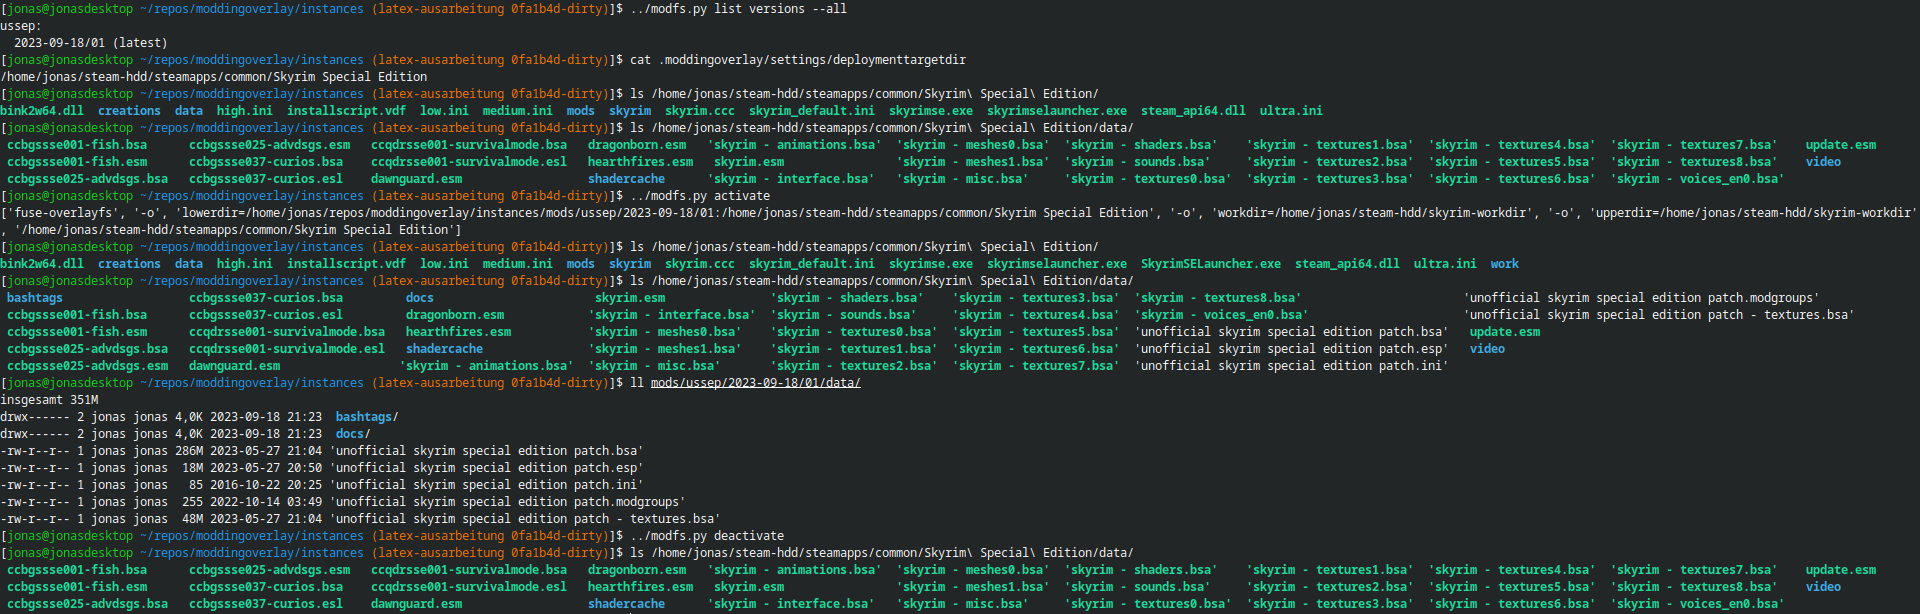
\includegraphics[width=\textwidth]{modfs-demo.png}}
  \caption{Demonstration von modfs in Aktion.
  Injizierung des unoffiziellen Fehlerbehebers (USSEP) in das Skyrim Special Edition Spielverzeichnis.}
  \label{fig:demo1}
\end{figure}

\begin{figure}
  \setlength{\fboxsep}{0pt}
  \setlength{\fboxrule}{.5pt}
  \fbox{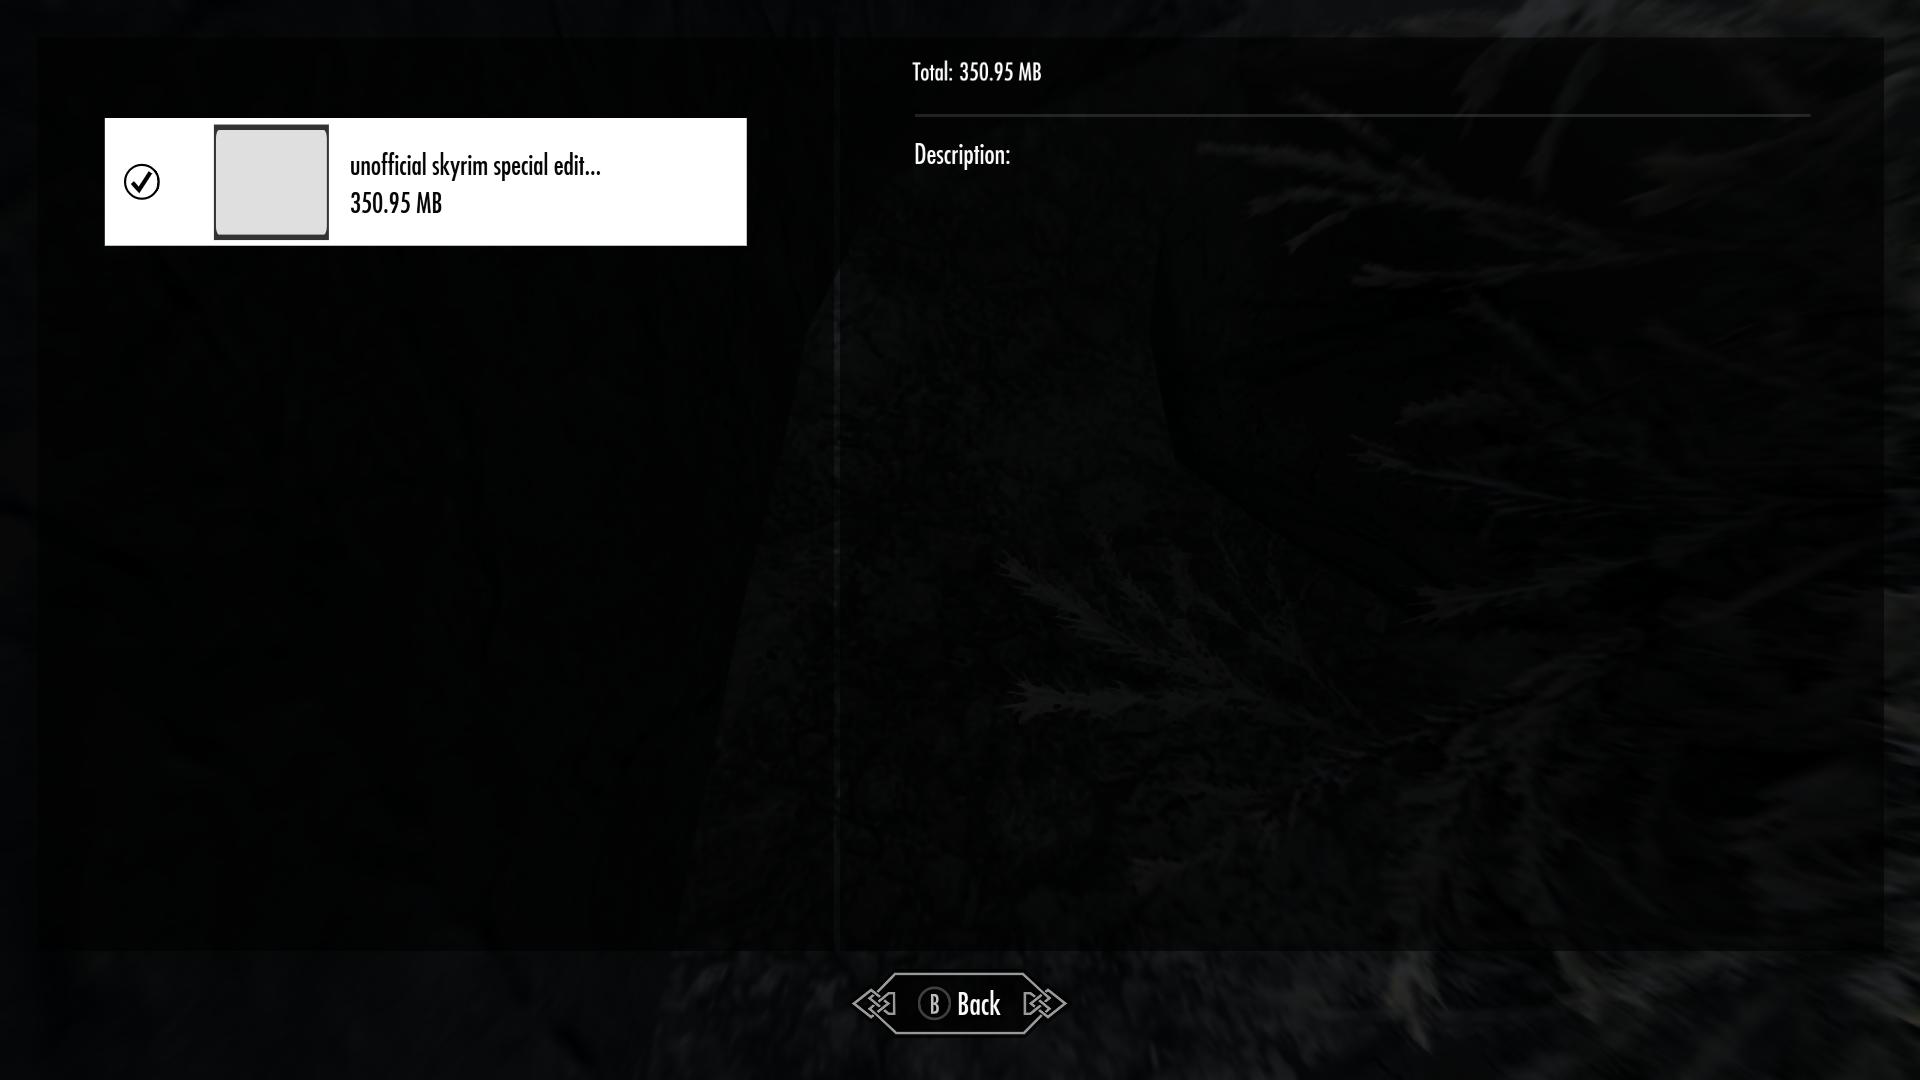
\includegraphics[width=\textwidth]{demo-mod-im-spiel.jpeg}}
  \caption{Ergebnis von modfs - der unoffizielle Fehlerbeheber in der Liste der geladenen Erweiterungen im laufenden Spiel}
  \label{fig:demo2}
\end{figure}

\begin{figure}
  \setlength{\fboxsep}{0pt}
  \setlength{\fboxrule}{.5pt}
  \fbox{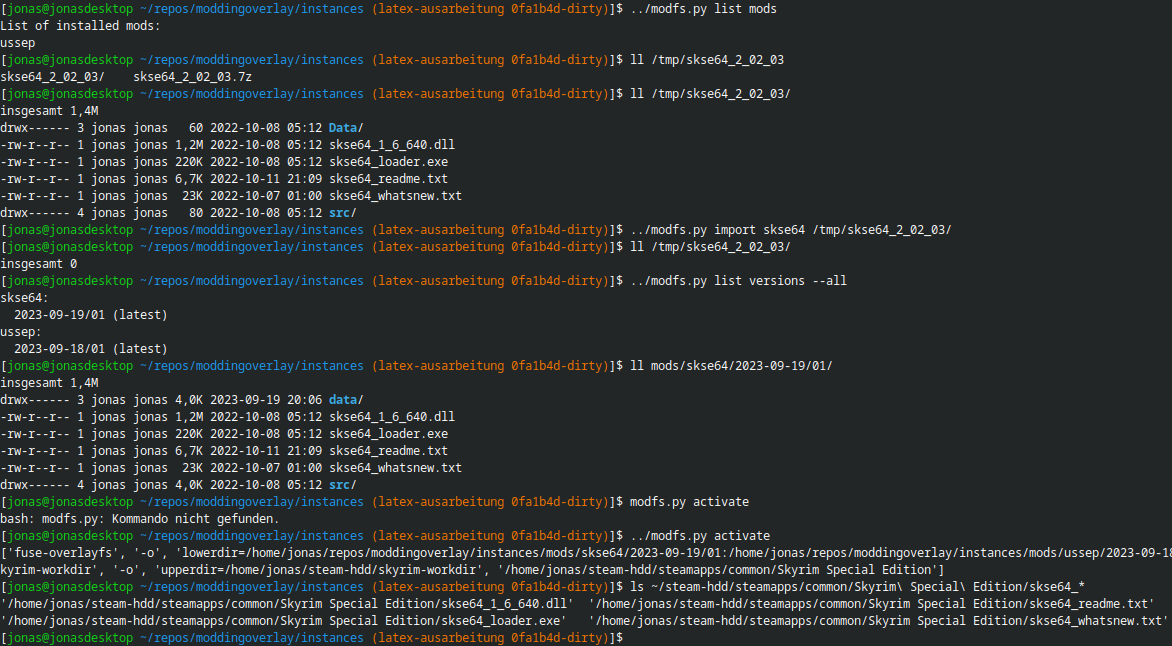
\includegraphics[width=\textwidth]{demo-import-mod.png}}
  \caption{Importieren einer neuen mod in modfs am Beispiel des Skyrim Script Extender (SKSE64)}
  \label{fig:demo_importmod}
\end{figure}

\end{document}
